% !TEX root = MAIN.tex

\chapter{Software Design Overview}

\section{Software static architecture}

Concerning the static architecture of the software we provide in the following descriptions for each of the components of the \FAQAS.

\subsection{Code-Driven Test Suite Evaluation}

\begin{figure}[h]
  \centering
	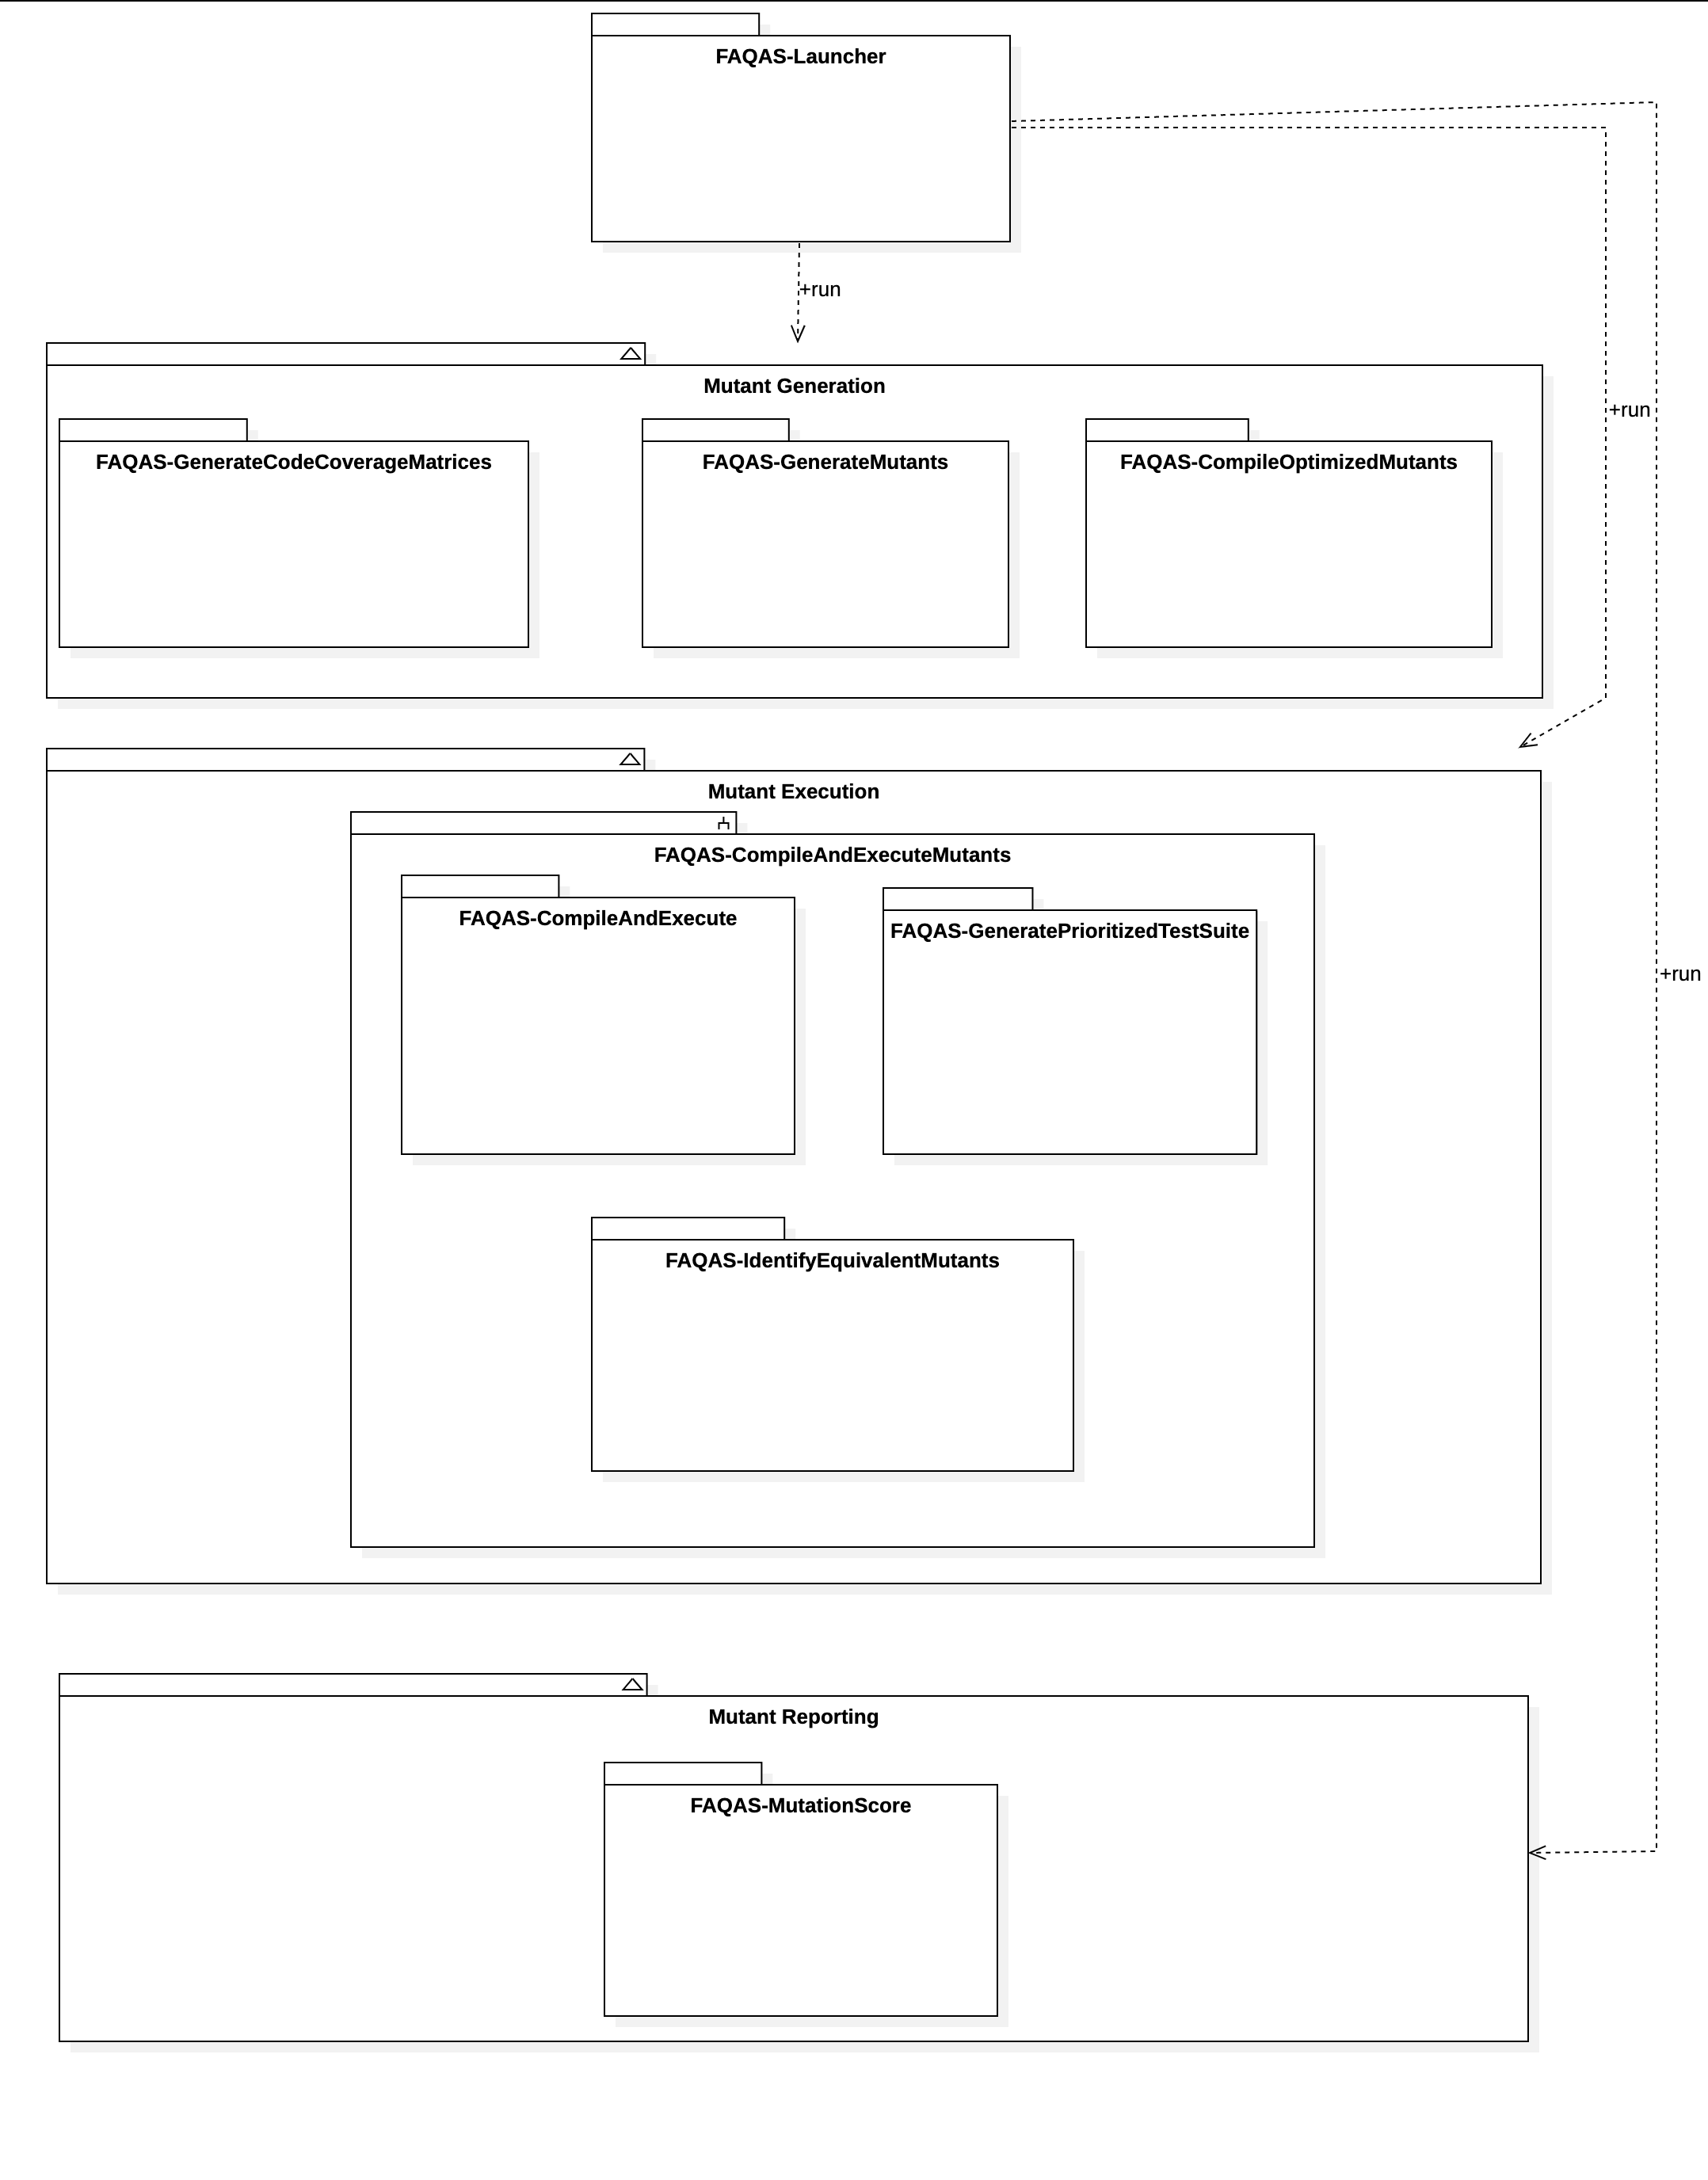
\includegraphics[width=0.8\textwidth]{images/static_architecture.png}
      \caption{UML Architecture diagram of the code-driven mutation testing component to evaluate test suite effectiveness.}
      \label{fig:architecture_diagram}
\end{figure}

The code-driven mutation testing component to evaluate test suite effectiveness is drafted in Figure~\ref{fig:architecture_diagram}.
Figure~\ref{fig:architecture_diagram} relies on UML package diagram notation. 

As depicted in Figure~\ref{fig:architecture_diagram}, the architecture of the component is divided in three layers. In particular, the architecture is composed by the \textit{Mutant Generation}, \textit{Mutant Execution}, and \textit{Mutant Reporting} layers, plus the entry point \textit{FAQAS-Launcher}. 

The layer \textit{Mutant Generation} implements the functionalities regarding the collection of code coverage, generation of mutants and discarding of equivalent and redundant mutants based on compiler optimisations.

The layer \textit{Mutant Execution} implements the functionalities regarding the compilation and execution of mutants. Note that this layer implements also the mutation sampling strategies and reduction of the test suite.

The layer \textit{Mutant Reporting} implements the functionalities regarding the computation of the mutation score and final reporting of the code-driven mutation process.

\begin{figure}[h]
  \centering
	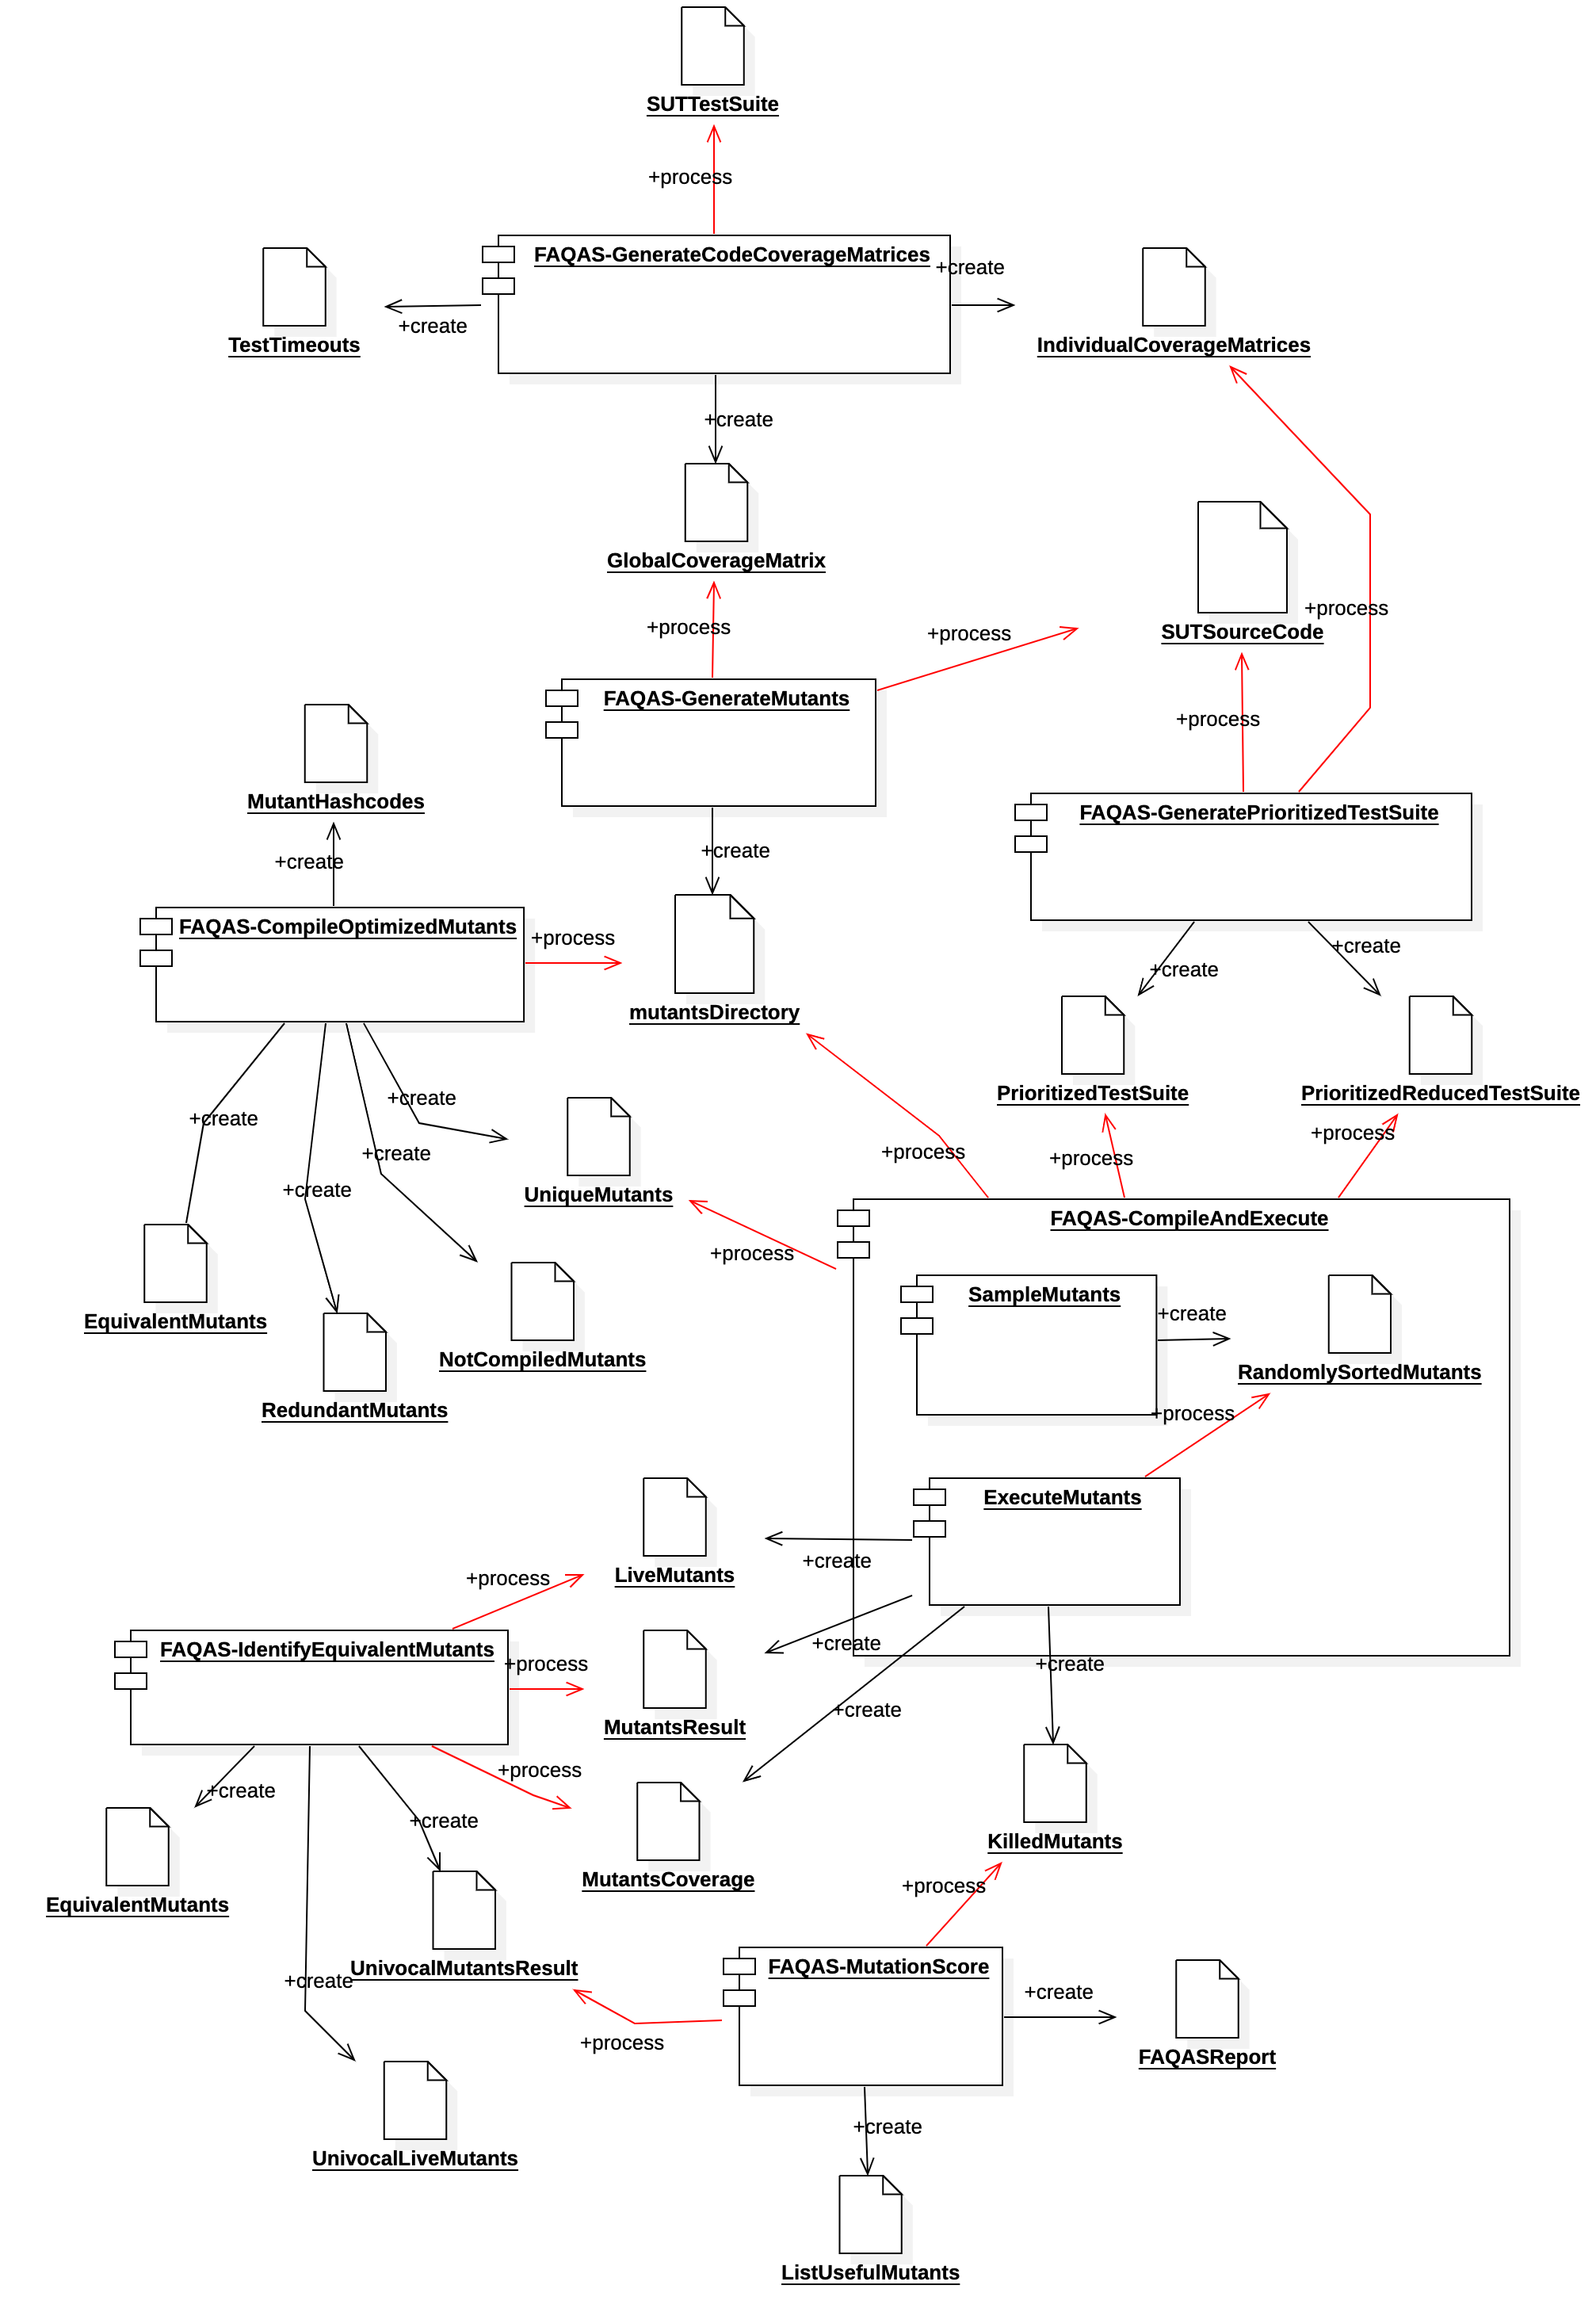
\includegraphics[width=0.9\textwidth]{images/component.png}
      \caption{UML Component diagram of the code-driven mutation testing component to evaluate test suite effectiveness.}
      \label{fig:component_diagram}
\end{figure}

The components of the code-driven mutation testing component to evaluate test suite effectiveness is drafted in Figure~\ref{fig:component_diagram}. Figure~\ref{fig:component_diagram} relies on UML component diagram notation.

As shown in Figure~\ref{fig:component_diagram}, the software is composed by the following components:

\begin{itemize}
	\item \textit{FAQAS-GenerateCodeCoverageMatrices}: this component processes the SUT test suite and generates the files \textit{GlobalCoverageMatrix}, \textit{IndividualCoverageMatrices}, and \textit{TestTimeouts}. The information produced by the component is mainly processed by the \textit{FAQAS-GenerateMutants} component.

	\item \textit{FAQAS-GenerateMutants}: This component processes the SUT source code, and the \textit{GlobalCoverageMatrix} file and generates the mutants directory.

	\item \textit{FAQAS-GeneratePrioritizedTestSuite}: this component processes the source code and the \textit{IndividualCoverageMatrices}, and produces two files: the \textit{PrioritizedTestSuite} and the \textit{PrioritizedReducedTestSuite}.

	\item \textit{FAQAS-CompileOptimizedMutants}: this component processes the mutants directory, and produces five files: 
	\begin{itemize}
		\item \textit{MutantHashcodes}: file containing the list of hash-codes for each mutant
		\item \textit{UniqueMutants}: file containing the list of nonequivalent and nonredundant mutants
		\item \textit{EquivalentMutants}: file containing the list of equivalent mutants
		\item \textit{RedundantMutants}: file containing the list of redundant mutants
		\item \textit{NotCompiledMutants}: file containing the list of non-compiled mutants
	\end{itemize}
	\item \textit{FAQAS-CompileAndExecute}: this component is composed by two sub-components:
		\begin{itemize}
			\item \textit{SampleMutants}: the component processes the file \textit{UniqueMutants} and generates the file \textit{RandomlySortedMutants}
			\item \textit{ExecuteMutants}: the component processes the file \textit{RandomlySortedMutants}, and execute the mutants producing the following files:
			\begin{itemize}
				\item \textit{LiveMutants}: file containing the list of live mutants
				\item \textit{KilledMutants}: file containing the list of killed mutants
				\item \textit{MutantsResults}: file containing the mutation traces
				\item \textit{MutantsCoverage}: folder containing the coverage for every mutant
			\end{itemize}
		\end{itemize}
	\item \textit{FAQAS-IdentifyEquivalentMutants}: this component processes the files \textit{LiveMutants}, \textit{MutantsResults}, and \textit{MutantsCoverage}, and generates the files \textit{EquivalentMutants}, \textit{UnivocalLiveMutants}, and \textit{UnivocalMutantsResults}, that is, it filters equivalent mutants from the mutation execution process.

	\item \textit{FAQAS-MutationScore}: this component processes the \textit{UnivocalMutantsResults} and the \textit{KilledMutants} files and produces the files \textit{FAQASReport} and \textit{LiveUsefulMutants}.
\end{itemize}


%\section{Software dynamic architecture}

\section{Software behavior}

Concerning the dynamic behavior of the software, we introduce in the following descriptions for each of the four components of the \FAQAS: the Code-Driven Test Suite Evaluation and Augmentation, and the Data-Driven Test Suite Evaluation and Augmentation.

\subsection{Code-Driven Test Suite Evaluation}

\begin{figure}[h]
  \centering
	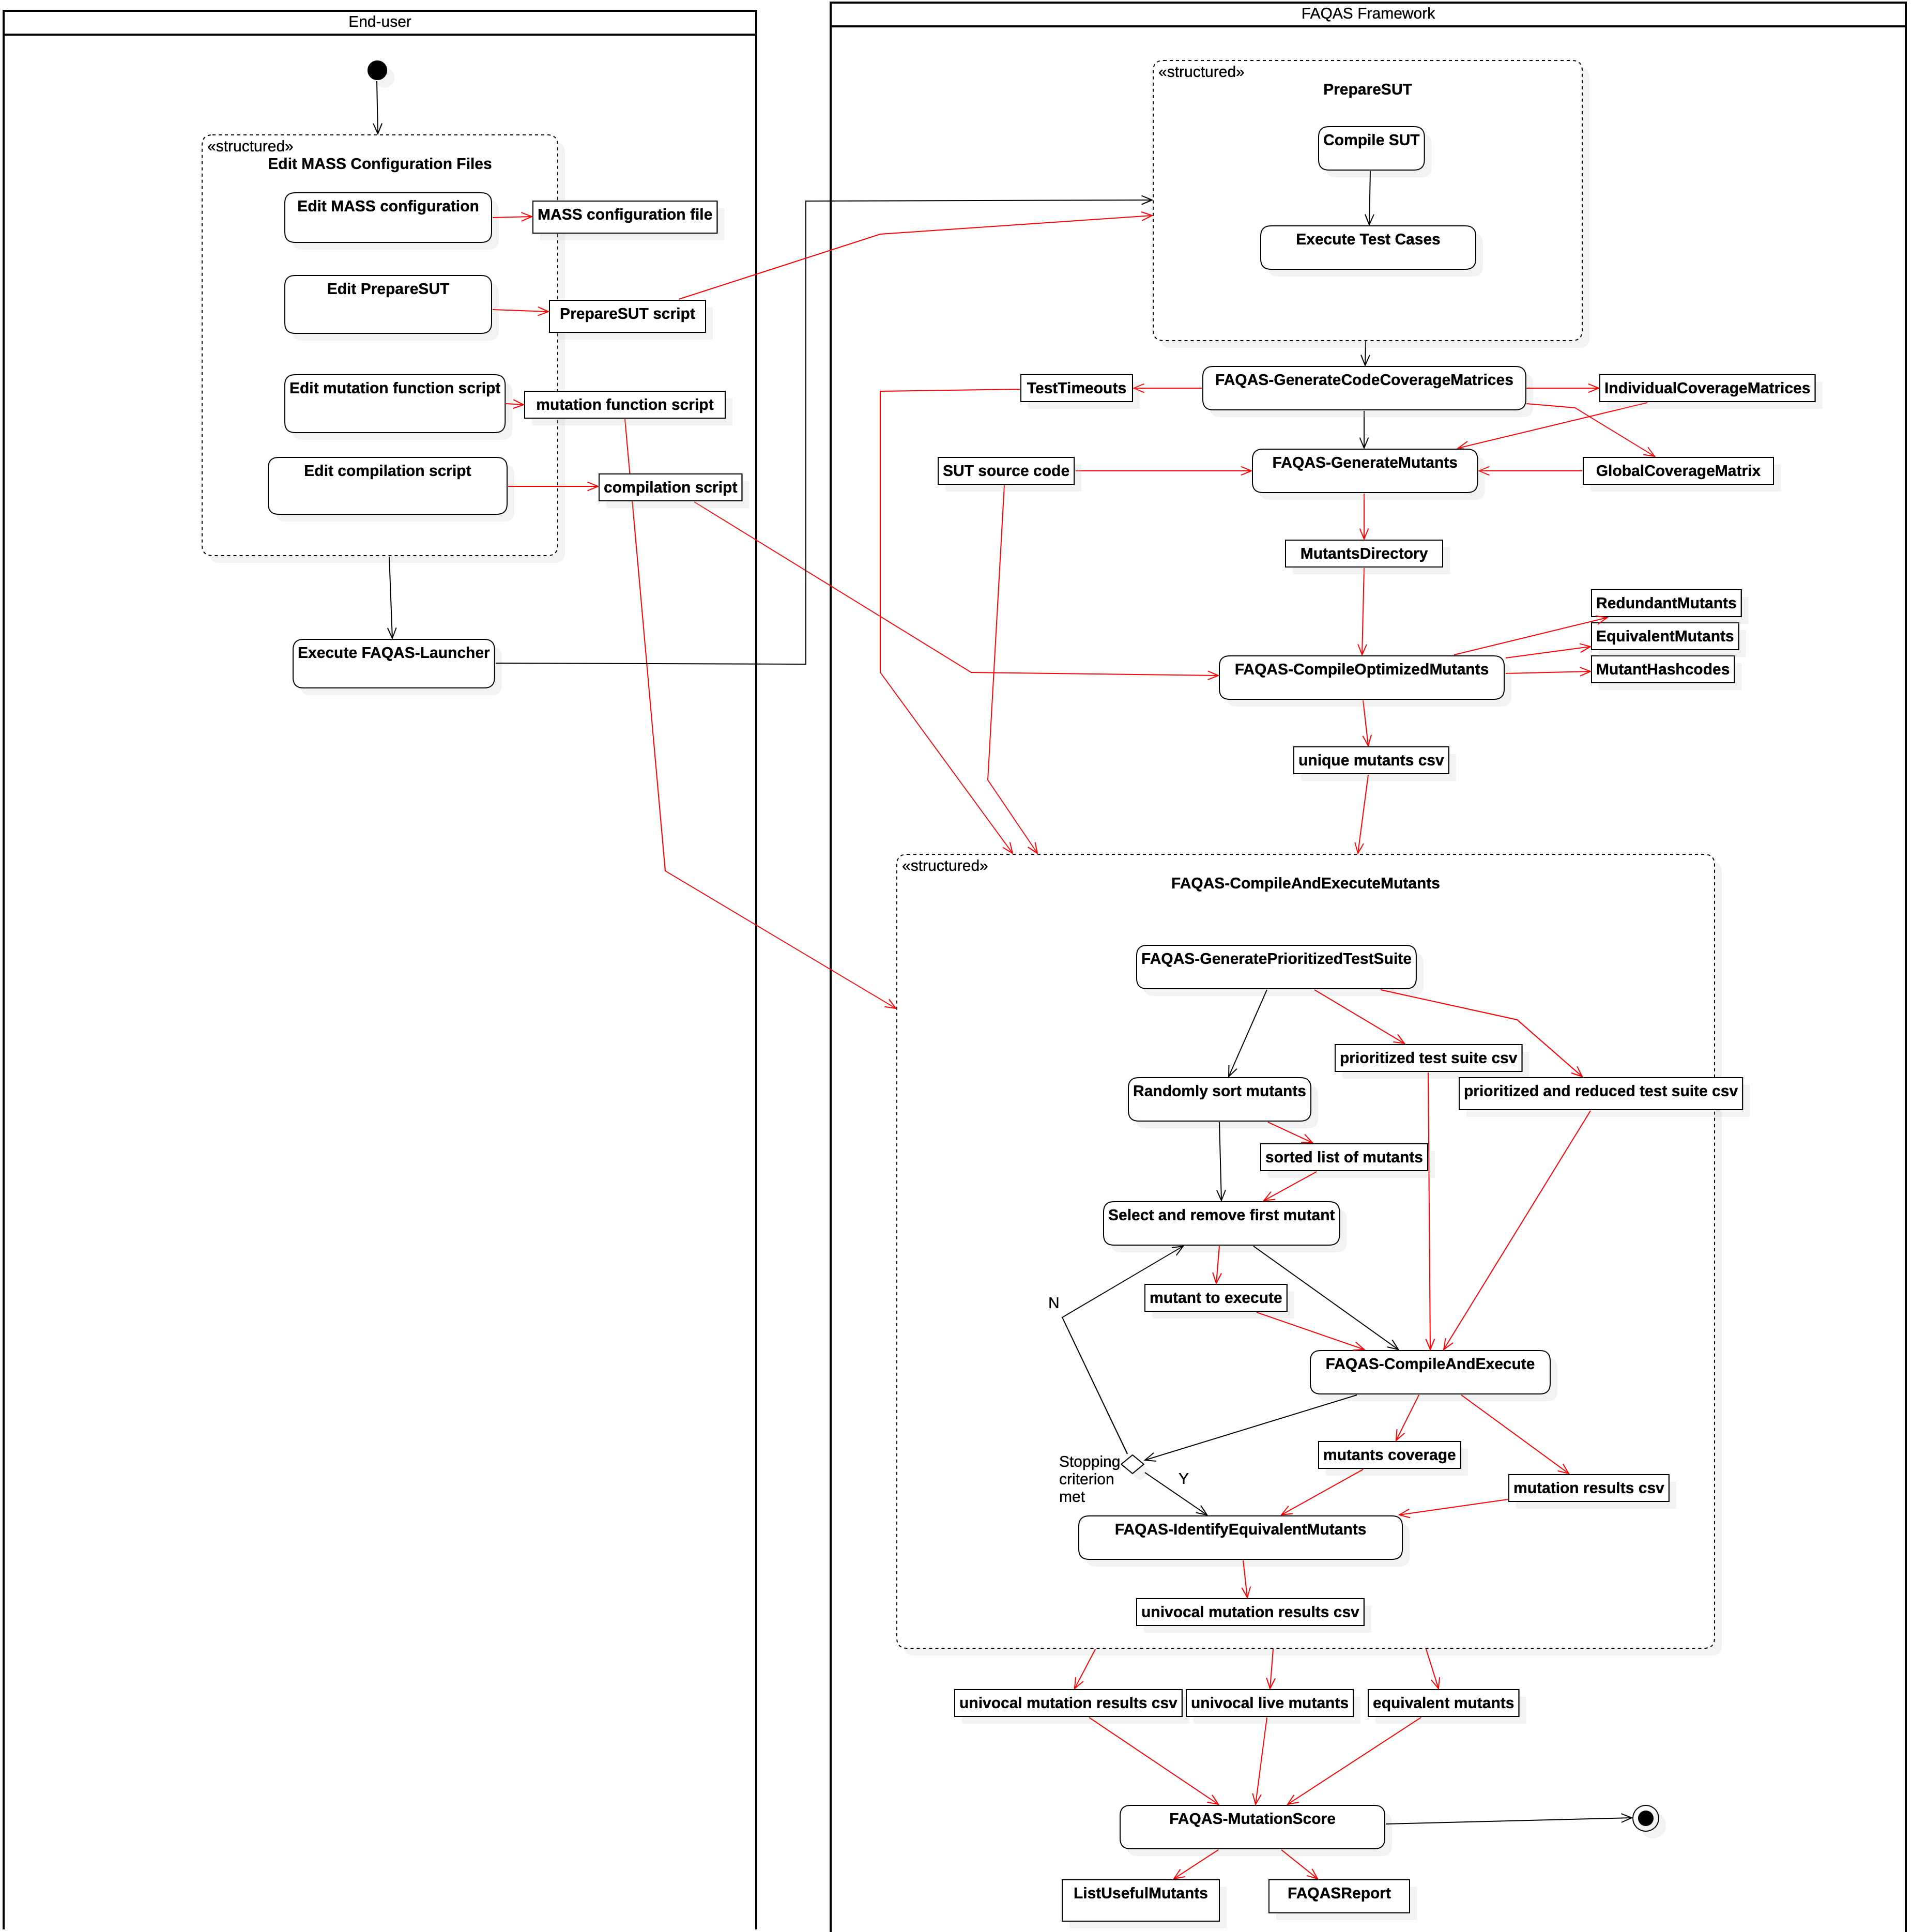
\includegraphics[width=\textwidth]{images/CodeDrivenTestSuiteEvaluation.png}
      \caption{Overview of the code-driven mutation testing process to evaluate test suite effectiveness.}
      \label{fig:process:codeDriven:evaluation}
\end{figure}


The code-driven mutation testing component implements the process for the evaluation of test suite effectiveness that is drafted in Figure~\ref{fig:process:codeDriven:evaluation}. Figure~\ref{fig:process:codeDriven:evaluation} relies on UML activity diagram notation. In Figure~\ref{fig:process:codeDriven:evaluation} the execution of specific software artefacts from the end user is made explicit. Also, we use black arrows to draw control-flow, red arrows for data-flow. In the following, we further describe the evaluation of test suite effectiveness process.


The activity \emph{Edit MASS Configuration Files} indicates that the engineers must configure the following files:
\begin{itemize}
	\item MASS configuration file: general configuration file
	\item PrepareSUT: script that compiles the SUT and executes the SUT test suite
	\item Mutation Function: implementation of the function that executes the SUT test cases and decides whether a test case has been killed.
	\item Compilation script: modified version of the original build script to be used by \emph{FAQAS-CompileOptimizedMutants}
\end{itemize}


The activity \emph{Compile SUT} in Figure~\ref{fig:process:codeDriven:evaluation} indicates that \MASS shall compile the SUT with coverage options enabled.

The activity \emph{Prepare test scripts} in Figure~\ref{fig:process:codeDriven:evaluation} concerns extending the \emph{test suite script} for the SUT to store the code coverage of each single test case separately. This is achieved by adding a call to a dedicated bash script provided by FAQAS (\emph{FAQAS-CollectCodeCoverage}) after the execution of every test case.

The activity \emph{Execute test cases} in Figure~\ref{fig:process:codeDriven:evaluation} concerns the execution of the test cases following the practice for the SUT (e.g., running the command \texttt{make test}).

The activity \emph{Execute FAQAS-GenerateCodeCoverageMatrix} in Figure~\ref{fig:process:codeDriven:evaluation} concerns the execution of a provided program delivered with the FAQAS framework.

The activity \emph{Execute FAQAS-GenerateCodeCoverageMatrix} in Figure~\ref{fig:process:codeDriven:evaluation} generates a set of files: 
\begin{itemize}
\item one csv file referred to as \emph{global coverage matrix}, which indicates, for every line of code of the SUT, the ID of the test cases that cover the line of code;
\item a number of files  referred to as \emph{individual coverage matrices}, one for each test case of the SUT. Each file indicates, for every line of code of the SUT, the number of times it has been covered during a single execution of the test case;
\item one file specifying, for each test case, a timeout value after which we shall consider a test case as hanging. The timeout value is generated by the system by triplicating the time taken by a test case launched in activity \emph{Execute test cases}.
\end{itemize}

Activity \emph{Execute FAQAS-GenerateMutants} in Figure~\ref{fig:process:codeDriven:evaluation} concerns the execution of the program \emph{FAQAS-GenerateMutants}. 

The program \emph{FAQAS-GenerateMutants} automatically generates a number of copies of each source file. Each copy contains one mutant.

\emph{FAQAS-GenerateMutants} mutates source files implemented with C programming languages.

\emph{FAQAS-GenerateMutants} generates mutants by applying a set of mutation operators that can be selected by the end-users.

\emph{FAQAS-GenerateMutants} implements the set of operators listed in Table~\ref{table:operators}

% !TEX root =  ../Main.tex

\newcommand{\op}{\mathit{op}}
\newcommand{\ArithmeticSet}{ \texttt{+}, \texttt{-}, \texttt{*}, \texttt{/}, \texttt{\%} }
\newcommand{\LogicalSet}{ \texttt{&&}, \texttt{||} }
\newcommand{\RelationalSet}{ \texttt{>}, \texttt{>=}, \texttt{<}, \texttt{<=}, \texttt{==}, \texttt{!=} }
\newcommand{\BitWiseSet}{ \texttt{\&}, \texttt{|}, \land }
\newcommand{\ShiftSet}{ \texttt{>>}, \texttt{<<} }


\begin{table}[h]
\caption{Implemented set of mutation operators.}
\label{table:operators} 
\centering
\scriptsize
\begin{tabular}{|@{}p{4mm}@{}|@{}p{2cm}@{\hspace{1pt}}|@{}p{11.1cm}@{}|}
\hline
&\textbf{Operator} & \textbf{Description$^{*}$} \\
\hline
\multirow{7}{*}{\rotatebox{90}{\emph{Sufficient Set}}}&ABS               & $\{(v, -v)\}$	\\
\cline{2-3}
&AOR               & $\{(\op_1, op_2) \,|\, \op_1, \op_2 \in \{ \ArithmeticSet \} \land \op_1 \neq \op_2 \} $       \\
&    			  & $\{(\op_1, \op_2) \,|\, \op_1, \op_2 \in \{\texttt{+=}, \texttt{-=}, \texttt{*=}, \texttt{/=}, \texttt{\%} \texttt{=}\} \land \op_1 \neq \op_2 \} $       \\
\cline{2-3}
&ICR               & $\{i, x) \,|\, x \in \{1, -1, 0, i + 1, i - 1, -i\}\}$           \\
\cline{2-3}
&LCR               & $\{(\op_1, \op_2) \,|\, \op_1, \op_2 \in \{ \texttt{\&\&}, || \} \land \op_1 \neq \op_2 \}$            \\
&				  & $\{(\op_1, \op_2) \,|\, \op_1, \op_2 \in \{ \texttt{\&=}, \texttt{|=}, \texttt{\&=}\} \land \op_1 \neq \op_2 \}$            \\
&				  & $\{(\op_1, \op_2) \,|\, \op_1, \op_2 \in \{ \texttt{\&}, \texttt{|}, \texttt{\&\&}\} \land \op_1 \neq \op_2 \}$            \\
\cline{2-3}
&ROR               & $\{(\op_1, \op_2) \,|\, \op_1, \op_2 \in \{ \RelationalSet \}\}$            \\
&				  & $\{ (e, !(e)) \,|\, e \in \{\texttt{if(e)}, \texttt{while(e)}\} \}$ \\
\cline{2-3}
&SDL               & $\{(s, \texttt{remove}(s))\}$            \\
\cline{2-3}
&UOI               & $\{ (v, \texttt{--}v), (v, v\texttt{--}), (v, \texttt{++}v), (v, v\texttt{++}) \}$            \\   
\hline
\hline
\multirow{5}{*}{\rotatebox{90}{\emph{OODL}}}&AOD               & $\{((t_1\,op\,t_2), t_1), ((t_1\,op\,t_2), t_2) \,|\, op \in \{ \ArithmeticSet \} $       \\ 
\cline{2-3}
&LOD               & $\{((t_1\,op\,t_2), t_1), ((t_1\,op\,t_2), t_2) \,|\, op \in \{  \} \}$       \\ 
\cline{2-3}
&ROD               & $\{((t_1\,op\,t_2), t_1), ((t_1\,op\,t_2), t_2) \,|\, op \in \{ \RelationalSet \} \}$       \\ 
\cline{2-3}
&BOD               & $\{((t_1\,op\,t_2), t_1), ((t_1\,op\,t_2), t_2) \,|\, op \in \{ \BitWiseSet \} \}$       \\ 
\cline{2-3}
&SOD               & $\{((t_1\,op\,t_2), t_1), ((t_1\,op\,t_2), t_2) \,|\, op \in \{ \ShiftSet \} \}$       \\ 
%\hline
%COR               & $\{(\op_1, \op_2) \,|\, \op_1, \op_2 \in \{ \texttt{\&\&}, \texttt{||}, \land \} \land \op_1 \neq \op_2 \}$            \\
\hline
\hline
\multirow{3}{*}{\rotatebox{90}{\emph{Other}}}&LVR			& $\{(l_1, l_2) \,|\, (l_1, l_2) \in \{(0,-1), (l_1,-l_1), (l_1, 0), (\mathit{true}, \mathit{false}), (\mathit{false}, \mathit{true})\}\}$\\
&&\\
&&\\
\hline
\end{tabular}

$^{*}$Each pair in parenthesis shows how a program element is modified by the mutation operator. Th eleft element of the pair is replaced with the right element. We follow standard syntax~\cite{kintis2018effective}. Program elements are literals ($l$), integer literals ($i$), boolean expressions ($e$), operators ($\op$), statements ($s$), variables ($v$), and terms ( $t_i$, which might be either variables or literals).
\end{table}

\emph{FAQAS-GenerateMutants} generates as output a directory tree (\emph{mutants directory} in Figure~\ref{fig:process:codeDriven:evaluation}) that follows the structure of the source directory tree of the SUT. However, every source file is replaced by a folder; the folder has the same name of the file. The folder contains all the mutants generated for that file. Every mutant has a name that univocally identifies it. The mutant name results from the conjunction of the following information:
source file name, mutated function name, mutated line, mutation operator name, mutation operation, mutated ``column'' (i.e., char position from the beginning of the line).
In the following, we report the structure of the output directory generated for a program

\begin{verbatim}
./src/store/vmem/vmem_checksum_first.c
./src/log/telemetry_appender.c

./src-mutants/store/vmem/vmem_checksum_first/
vmem_checksum_first.mut.145.7_1_13.ROR.vmem_param_load.c
./src-mutants/log/telemetry_appender/
telemetry_appender.mut.116.3_1_18.ROR.gs_log_appender_telem_append_isr.c
\end{verbatim}


Activity \emph{Prepare compilation scripts} in Figure~\ref{fig:process:codeDriven:evaluation} concerns applying the modified build script for the SUT (e.g., the \emph{Makefile}). The file must be modified by:
\begin{itemize}
\item Removing debugging flags
\item Removing coverage flags
\item Adding a placeholder for the compiler optimization option
\item Adding a 'sort' command in the source dependency list to ensure that source files are always compiled in the same order
\end{itemize}


Activity \emph{Execute FAQAS-CompileOptimizedMutants} in Figure~\ref{fig:process:codeDriven:evaluation} concerns the execution of the program \emph{FAQAS-CompileOptimizedMutants}.

The program \emph{FAQAS-CompileOptimizedMutants} compiles every mutant multiple times, once for every compiler optimization option selected by the end-user. It implements the pseudocode in Figure~\ref{alg:CompileOptimizedMutants}.

\begin{figure}[h]
\begin{algorithmic}[1]

%\footnotesize
\scriptsize

\Require \emph{OPT}, the set of compiler optimization options specified by the end-user
\Require \emph{MutantsDir}, path of the directory tree containing the mutants
\Require \emph{SUTsources}, path of the folder containing the sources of the SUT
\Require \emph{CompilatonCommand}, the command to execute to compile the original software

\Ensure \emph{hashcodes csv}, a csv file containing for every mutant, for every option, the SHA512 hashcode of the generated executable

\Ensure \emph{unique mutants}, a csv file containing the list of unique mutants. Unique mutants are mutants that are not equivalent and not redundant. See D2 for details.

\For {OPT in OPTS}
\For {Mutant in MutantsDir}
\State Compile \emph{Mutant} with program \emph{FAQAS-CompileAndExecute}
\State Generate a SHA512 hash of the generated executable
\State Put the generated SHA512 hash in the \emph{hashcodes csv} file
\EndFor
\EndFor

\State Process \emph{hashcodes csv} and identify the \emph{unique mutants}
\State Save the list of \emph{unique mutants} in the output file \emph{unique mutants csv} 

\end{algorithmic}
\caption{FAQAS-CompileOptimizedMutants: Algorithm for compiling mutants with multiple optimization options}
\label{alg:CompileOptimizedMutants}
\end{figure}


Activity \emph{Execute FAQAS-CompileAndExecuteMutants} in Figure~\ref{fig:process:codeDriven:evaluation} concerns the execution of the program \emph{FAQAS-CompileAndExecuteMutants}.

The program \emph{FAQAS-CompileAndExecuteMutants} iterates over three activities: \emph{FAQAS-GeneratePrioritizedTestSuite}, \emph{FAQAS-CompileAndExecute}, \emph{FAQAS-IdentifyEquivalentMutants}. Each activity is implemented by a dedicated executable program that is invoked automatically by \emph{FAQAS-CompileAndExecuteMutants} without user intervention.

The program \emph{FAQAS-CompileAndExecuteMutants} takes as inputs the \emph{mutants selection configuration}, the \emph{unique mutants csv}, the path of the \emph{SUT source folder}, the \emph{command to execute test cases}, and the \emph{path to the folder containing the test coverage matrices}.

The program \emph{FAQAS-CompileAndExecuteMutants} implements the four mutants selection strategies described in D2: \emph{all mutants}, \emph{proportional uniform sampling}, \emph{proportional method-based sampling}, \emph{uniform fixed-size sampling}, and \emph{uniform FSCI sampling}.

The \emph{mutants sampling configuration} consists of the mutants selection strategy and a configuration value that specifies the number of mutants to consider. The format of the value that specifies the number of mutants to consider depends on the strategy; the value may indicate the percentage of mutants to sample (for \emph{proportional uniform sampling}, \emph{proportional method-based sampling}), the number of mutants to sample (for \emph{uniform fixed-size sampling}).

The program\emph{FAQAS-GeneratePrioritizedTestSuite} takes as input the test coverage matrices and generates a file that specifies, for every line of the SUT, the prioritized list of test cases to execute (\emph{prioritized test suite csv}). This file indicates the sequence of test cases that shall be executed when testing a mutant affecting a certain line.

The activity \emph{Randomly sort mutants} indicates that  \emph{FAQAS-CompileAndExecuteMutants} generates a randomly sorted list of mutants. The list contains the mutants in \emph{unique mutants csv}.
In the case of \emph{proportional method-based sampling}, the list contains a set of mutants selected by following the stratified sampling strategy.

The activity \emph{Select and remove first mutant} indicates that  \emph{FAQAS-CompileAndExecuteMutants} selects the first mutant in \emph{sorted list of mutants} and removes it from the list.

The program \emph{FAQAS-CompileAndExecute} compiles a mutant by running the build script of the original program; then it executes the SUT test suite. It follows the algorithm in Figure~\ref{alg:compileAndExecute}.


\begin{figure}[h]
\begin{algorithmic}[1]
\scriptsize
\Require \emph{Mutant}, path of the mutant to compile
\Require \emph{SUTsources}, path of the folder containing the sources of the SUT
\Require \emph{CompilatonCommand}, the command to execute to compile the original software
\Require \emph{TestCommand}, the command to execute to execute a single test case
\Require \emph{TestCases}, the prioritized list of test cases for the line of the mutant
\Require \emph{TestTimeout}, the max execution time that can be taken by the test case
\Ensure \emph{Result} KILLED or LIVE, based on test execution result (i.e., all test cases pass or one test case fails)
\State put \emph{Mutant} in place of the file it has been derived (\emph{original file}), keep the original file in a safe place
\State execute  \emph{CompilatonCommand} inside \emph{SUTsources}
\For {TestCase in TestCases}
\State execute the \emph{TestCase} by running \emph{TestCommand} inside \emph{SUTsources}
% succede qualcosa strano quando scrivi "the"
\If {the \emph{TestCase} fails (i.e., \emph{TestCommand} terminates with an error code)}
\State set \emph{Result} as KILLED
\State break the for loop
\EndIf
\If {the \emph{TestTimeout} expires}
\State set \emph{Result} as KILLED
\State break the for loop
\EndIf
\EndFor
\State move code coverage information in a subfolder of \emph{mutants coverage dir}
\State restore the \emph{original file}
\end{algorithmic}
\caption{FAQAS-CompileAndExecute: Algorithm to compile and test mutants}
\label{alg:compileAndExecute}
\end{figure}

The program \emph{FAQAS-CompileAndExecute} collects the mutation results of every mutant in a file, i.e., \emph{mutation results csv}. It contains, for every mutant, the indication of the mutation result (KILLED/LIVE).

The program \emph{FAQAS-CompileAndExecute} compiles and executes mutants till a termination criterion is met. The termination criterion depends on the mutants selection strategy (see D2 for details):
\begin{itemize}
\item \emph{all mutants}: the list \emph{sorted list of mutants} is empty
\item \emph{proportional uniform sampling}: a number of mutants matching the selected percentage has been executed
\item \emph{proportional method-based sampling}: the list \emph{sorted list of mutants} is empty
\item \emph{uniform fixed-size sampling}: a number of mutants matching the selected value has been executed
\item \emph{uniform FSCI sampling}: the confidence interval computed from \emph{mutation results csv} is smaller than the length specified by the user.
\end{itemize}

The program \emph{FAQAS-IdentifyEquivalentMutants} relies on code coverage information stored in \emph{mutants coverage dir} to identify equivalent and redundant mutants using the distance criterion $D_C$ (see D2).

The program \emph{FAQAS-IdentifyEquivalentMutants} generates a copy of \emph{mutation results csv} (i.e., \emph{univocal mutation results csv}) where only mutants that are considered non-equivalent are reported.

The program \emph{FAQAS-MutationScore} concerns the computation of the mutation score based on the mutation results reported in \emph{univocal mutation results csv}, and the production of two lists of useful mutants of live and nonequivalent mutants.


\subsection{Code-Driven Test Suite Augmentation}

The activity \emph{Execute FAQAS-CompileAndExecuteMutants} in Figure~\ref{fig:process:codeDriven:augmentation} concerns the execution of the program \emph{FAQAS-GenerateTestGenerationScaffolding}.

\begin{figure}[h]
  \centering
	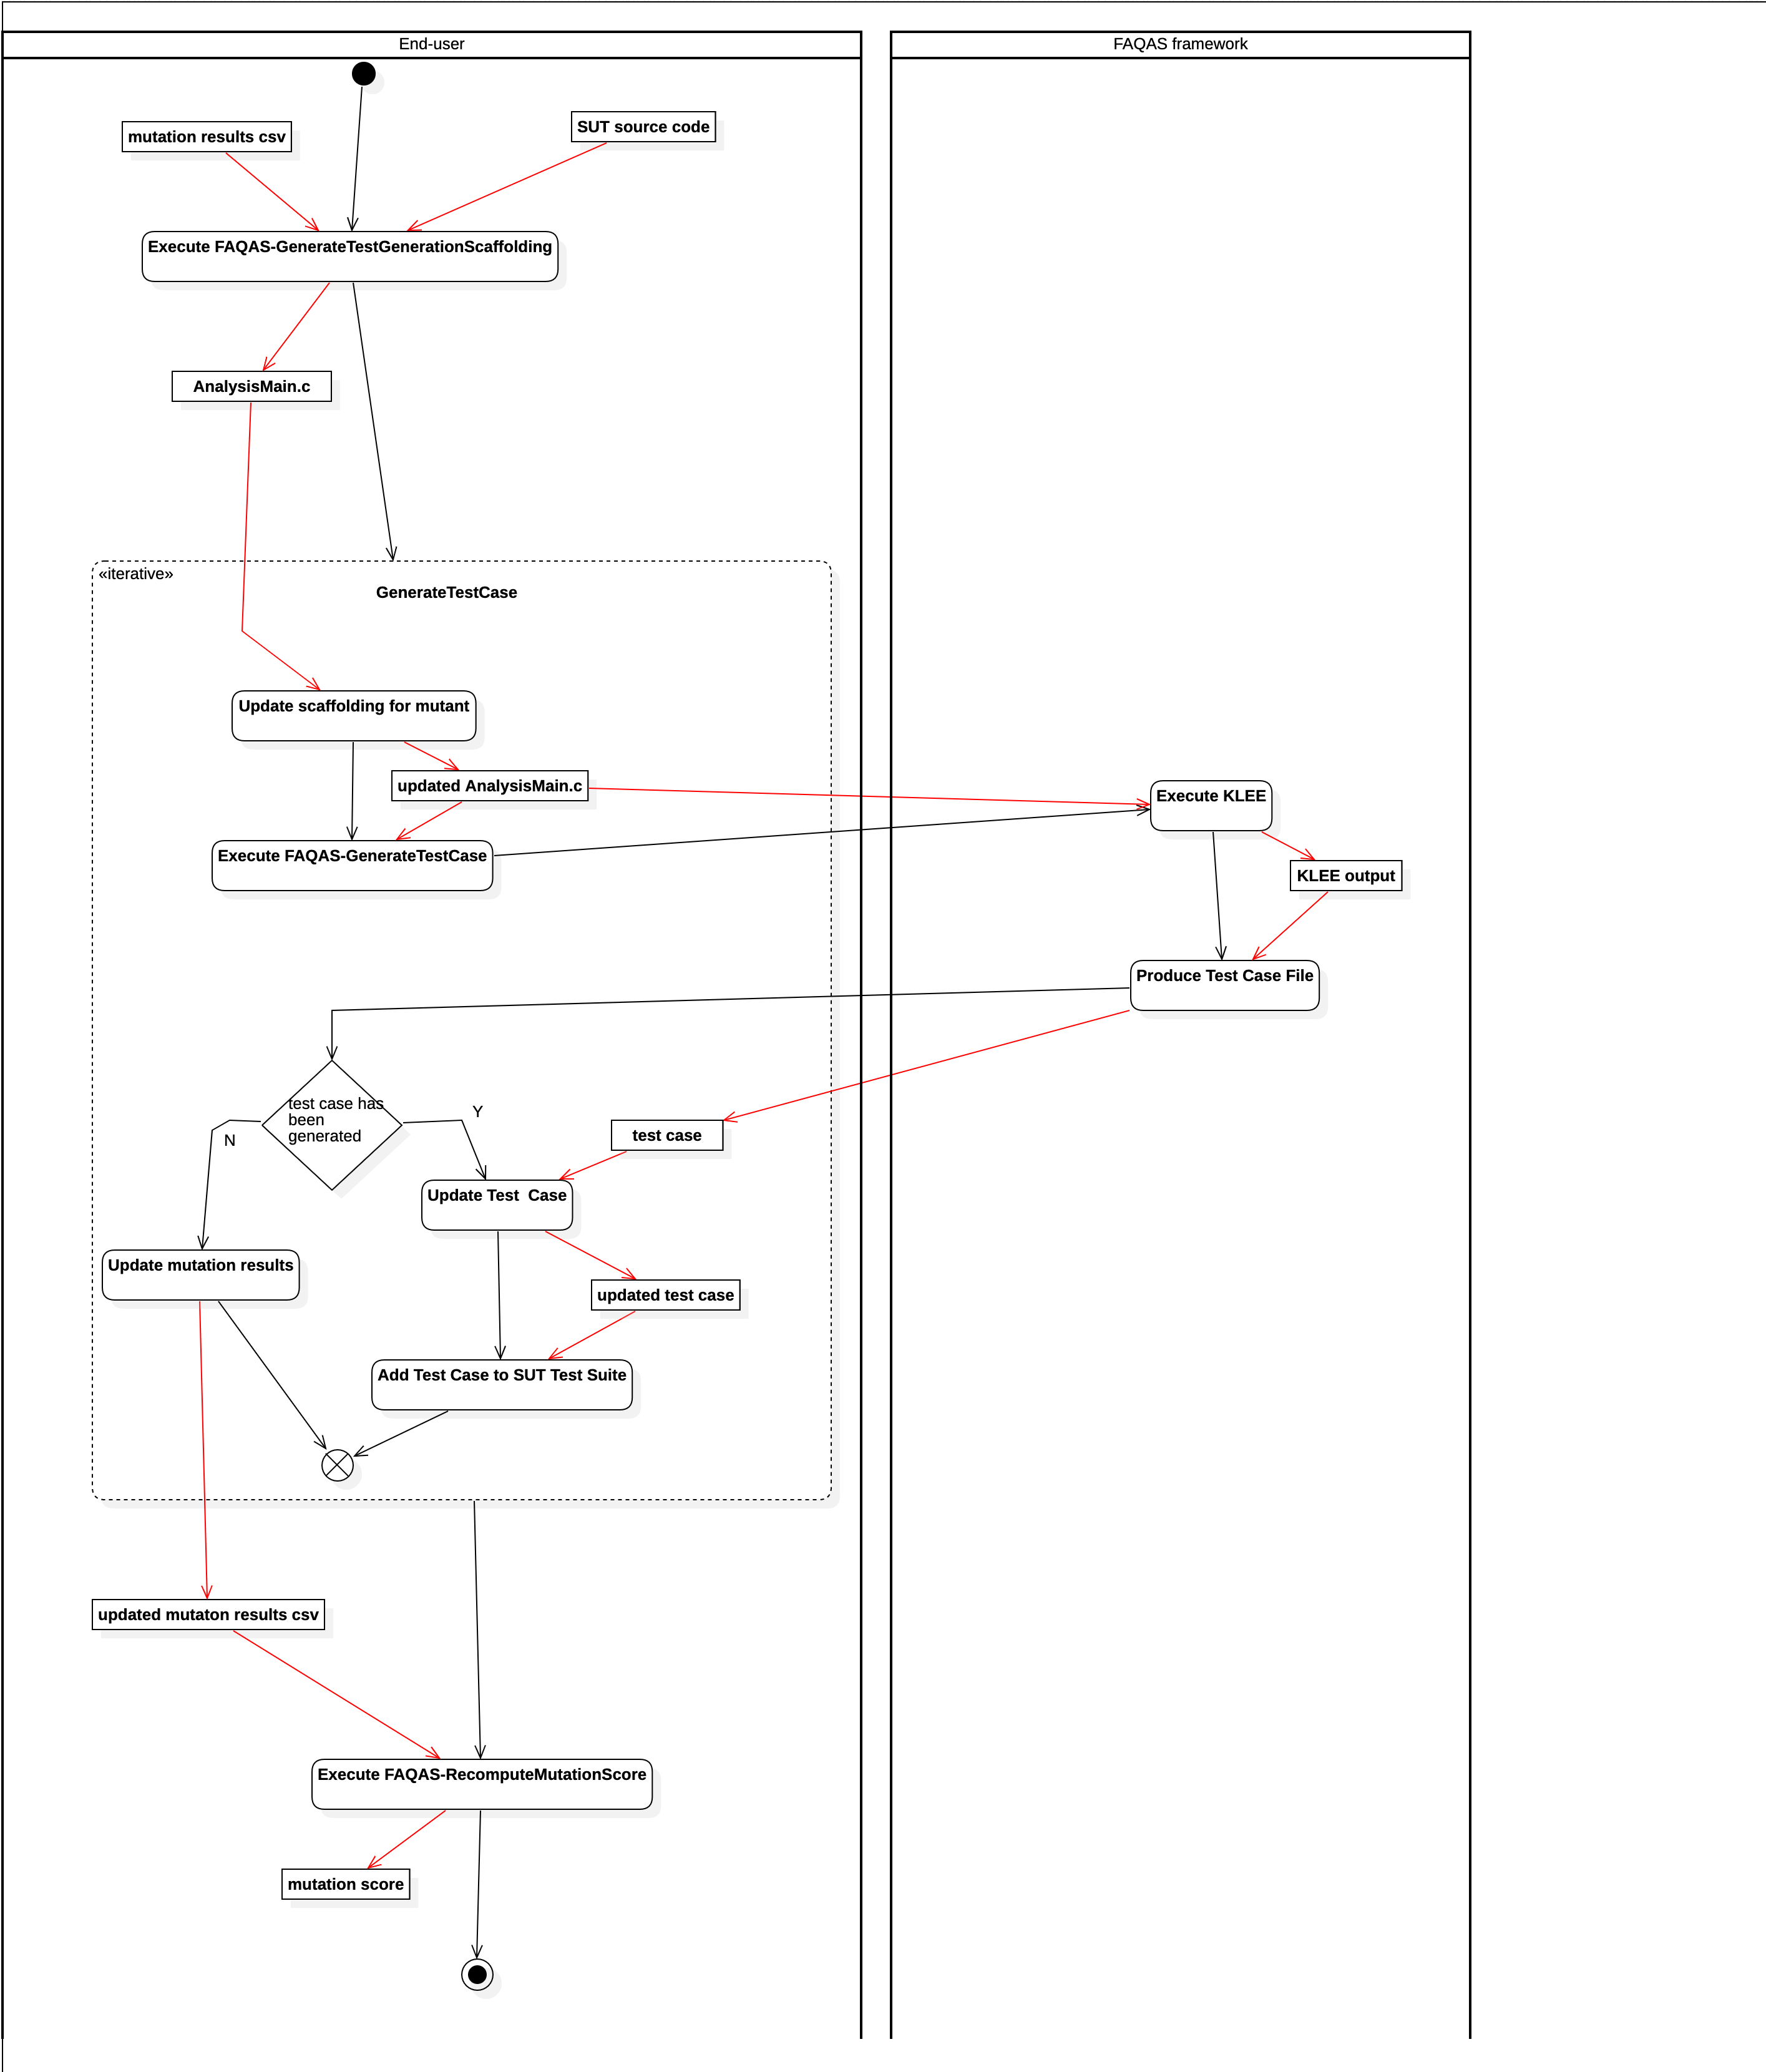
\includegraphics[width=\textwidth]{images/png/Activity1!CodeDrivenTestSuiteAugmentation_2.png}
      \caption{Overview of the code-driven test suite augmentation process.}
      \label{fig:process:codeDriven:augmentation}
\end{figure}

The code-driven mutation testing component also implements the process for the improvement of the effectiveness of test suites that is drafted in Figure~\ref{fig:process:codeDriven:augmentation}. Figure~\ref{fig:process:codeDriven:augmentation} relies on UML activity diagram notation. In Figure~\ref{fig:process:codeDriven:augmentation} the execution of specific software artefacts from the end user is made explicit. Also, we use black arrows to draw control-flow, red arrows for data-flow.

The program \emph{FAQAS-GenerateTestGenerationScaffolding} takes as input the path of the \emph{SUT source code} and the file \emph{mutation results csv}. It generates a number of files named \emph{MutantId\_AnalysisMain.c}, one for each live mutant, where MutantId is the ID of a mutant. The file \emph{MutantId\_AnalysisMain.c} contains a main function that should be used for the analysis with KLEE. 

The content of file \emph{MutantId\_AnalysisMain.c} should resemble \emph{Listing 1.7} and \emph{Listing 1.9} of D2, it should enable the analysis with KLEE. For example, it should import the source file with the original function targeted by the mutation and the source code of the mutated function. Also, it should contain the definition of all the variables used for the execution of KLEE and a tentative set of required assertions.

The activity \emph{Update scaffolding for mutant} in Figure~\ref{fig:process:codeDriven:augmentation} indicates that the engineer should modify the file  \emph{MutantId\_AnalysisMain.c} if necessary. In particular, it might be necessary to refine the assertions produced by \emph{FAQAS-GenerateTestGenerationScaffolding}. More precisely, since assertions should concern output variables, it is necessary to verify that all the necessary output variables had been referred in assertion. Indeed, in C, with pointers and pointers to pointers, it is not possible to have a precise automated identification of output variables.

The activities in the expansion region \emph{generateTestCase} are repeated for every live mutant.

The activity \emph{Execute FAQAS-GenerateTestCase} in Figure~\ref{fig:process:codeDriven:augmentation} concerns the execution of the program \emph{FAQAS-GenerateTestCase}.

The program \emph{FAQAS-GenerateTestCase} generates a tentative unit test case (i.e., a source file in C) that kills the mutant. It executes the KLEE program and then produces a unit test case (i.e., a file with a main in C) after processing the KLEE output.

For test generation, the support for the programming language of the SUT depends on KLEE (it supports C, limited support for C++).

The test case generated by \emph{FAQAS-GenerateTestCase} contains an invocation of the function under test (i.e., the function targeted  by the mutation) along with assigned arguments and an assertion that verifies results. The values for the assigned arguments and the verification of results are derived from the output of KLEE.

If the program \emph{FAQAS-GenerateTestCase} successfully generates a test case, the engineer proceeds with inspecting it (activity \emph{Update Test  Case}), otherwise he can consider the mutant as equivalent (activity \emph{Update mutation results}).

The activity \emph{Update Test  Case} in Figure~\ref{fig:process:codeDriven:augmentation} is performed by the engineer. He may need to execute the generated test case to verify that KLEE has generated valid inputs (e.g., inputs that meet the program preconditions). Based on KLEE results, \emph{FAQAS-GenerateTestCase} also generates assertions that reflect the output observed by KLEE (e.g., \texttt{assert( output == value\_observed\_by\_KLEE)} ). The engineer should thus also verify that the assertion with the expected value is correct (i.e., it reflects what indicated in the SUT specifications). If the value appearing in the assertion is not correct, it means that KLEE during its execution has observed an incorrect value being generated by the SUT; for this reason, the SUT might be faulty and should be fixed.

The activity \emph{Add Test Case to SUT Test Suite} in Figure~\ref{fig:process:codeDriven:augmentation} is performed by the engineer, who may add the new test case to the test suite.

The activity \emph{Update mutation results} in Figure~\ref{fig:process:codeDriven:augmentation} is performed when a test case is not generated. This generally happens when the mutant cannot be killed (i.e., is equivalent). The engineer is expected to manually inspect the mutant to be sure that the mutant is equivalent (otherwise the missing test case is due to a limitation of KLEE). If the mutant is equivalent the engineer removes it from the file \emph{mutation results csv}.

The activity \emph{Execute FAQAS-RecomputeMutationScore} in Figure~\ref{fig:process:codeDriven:augmentation}  concerns the execution of the program \emph{FAQAS-RecomputeMutationScore}. It is performed after generating test cases for all the live mutants. Program \emph{FAQAS-RecomputeMutationScore} recomputes the mutation score after ignoring the equivalent mutants detected by KLEE.


\subsection{Data-Driven Test Suite Evaluation}

\begin{figure}[h]
  \centering
	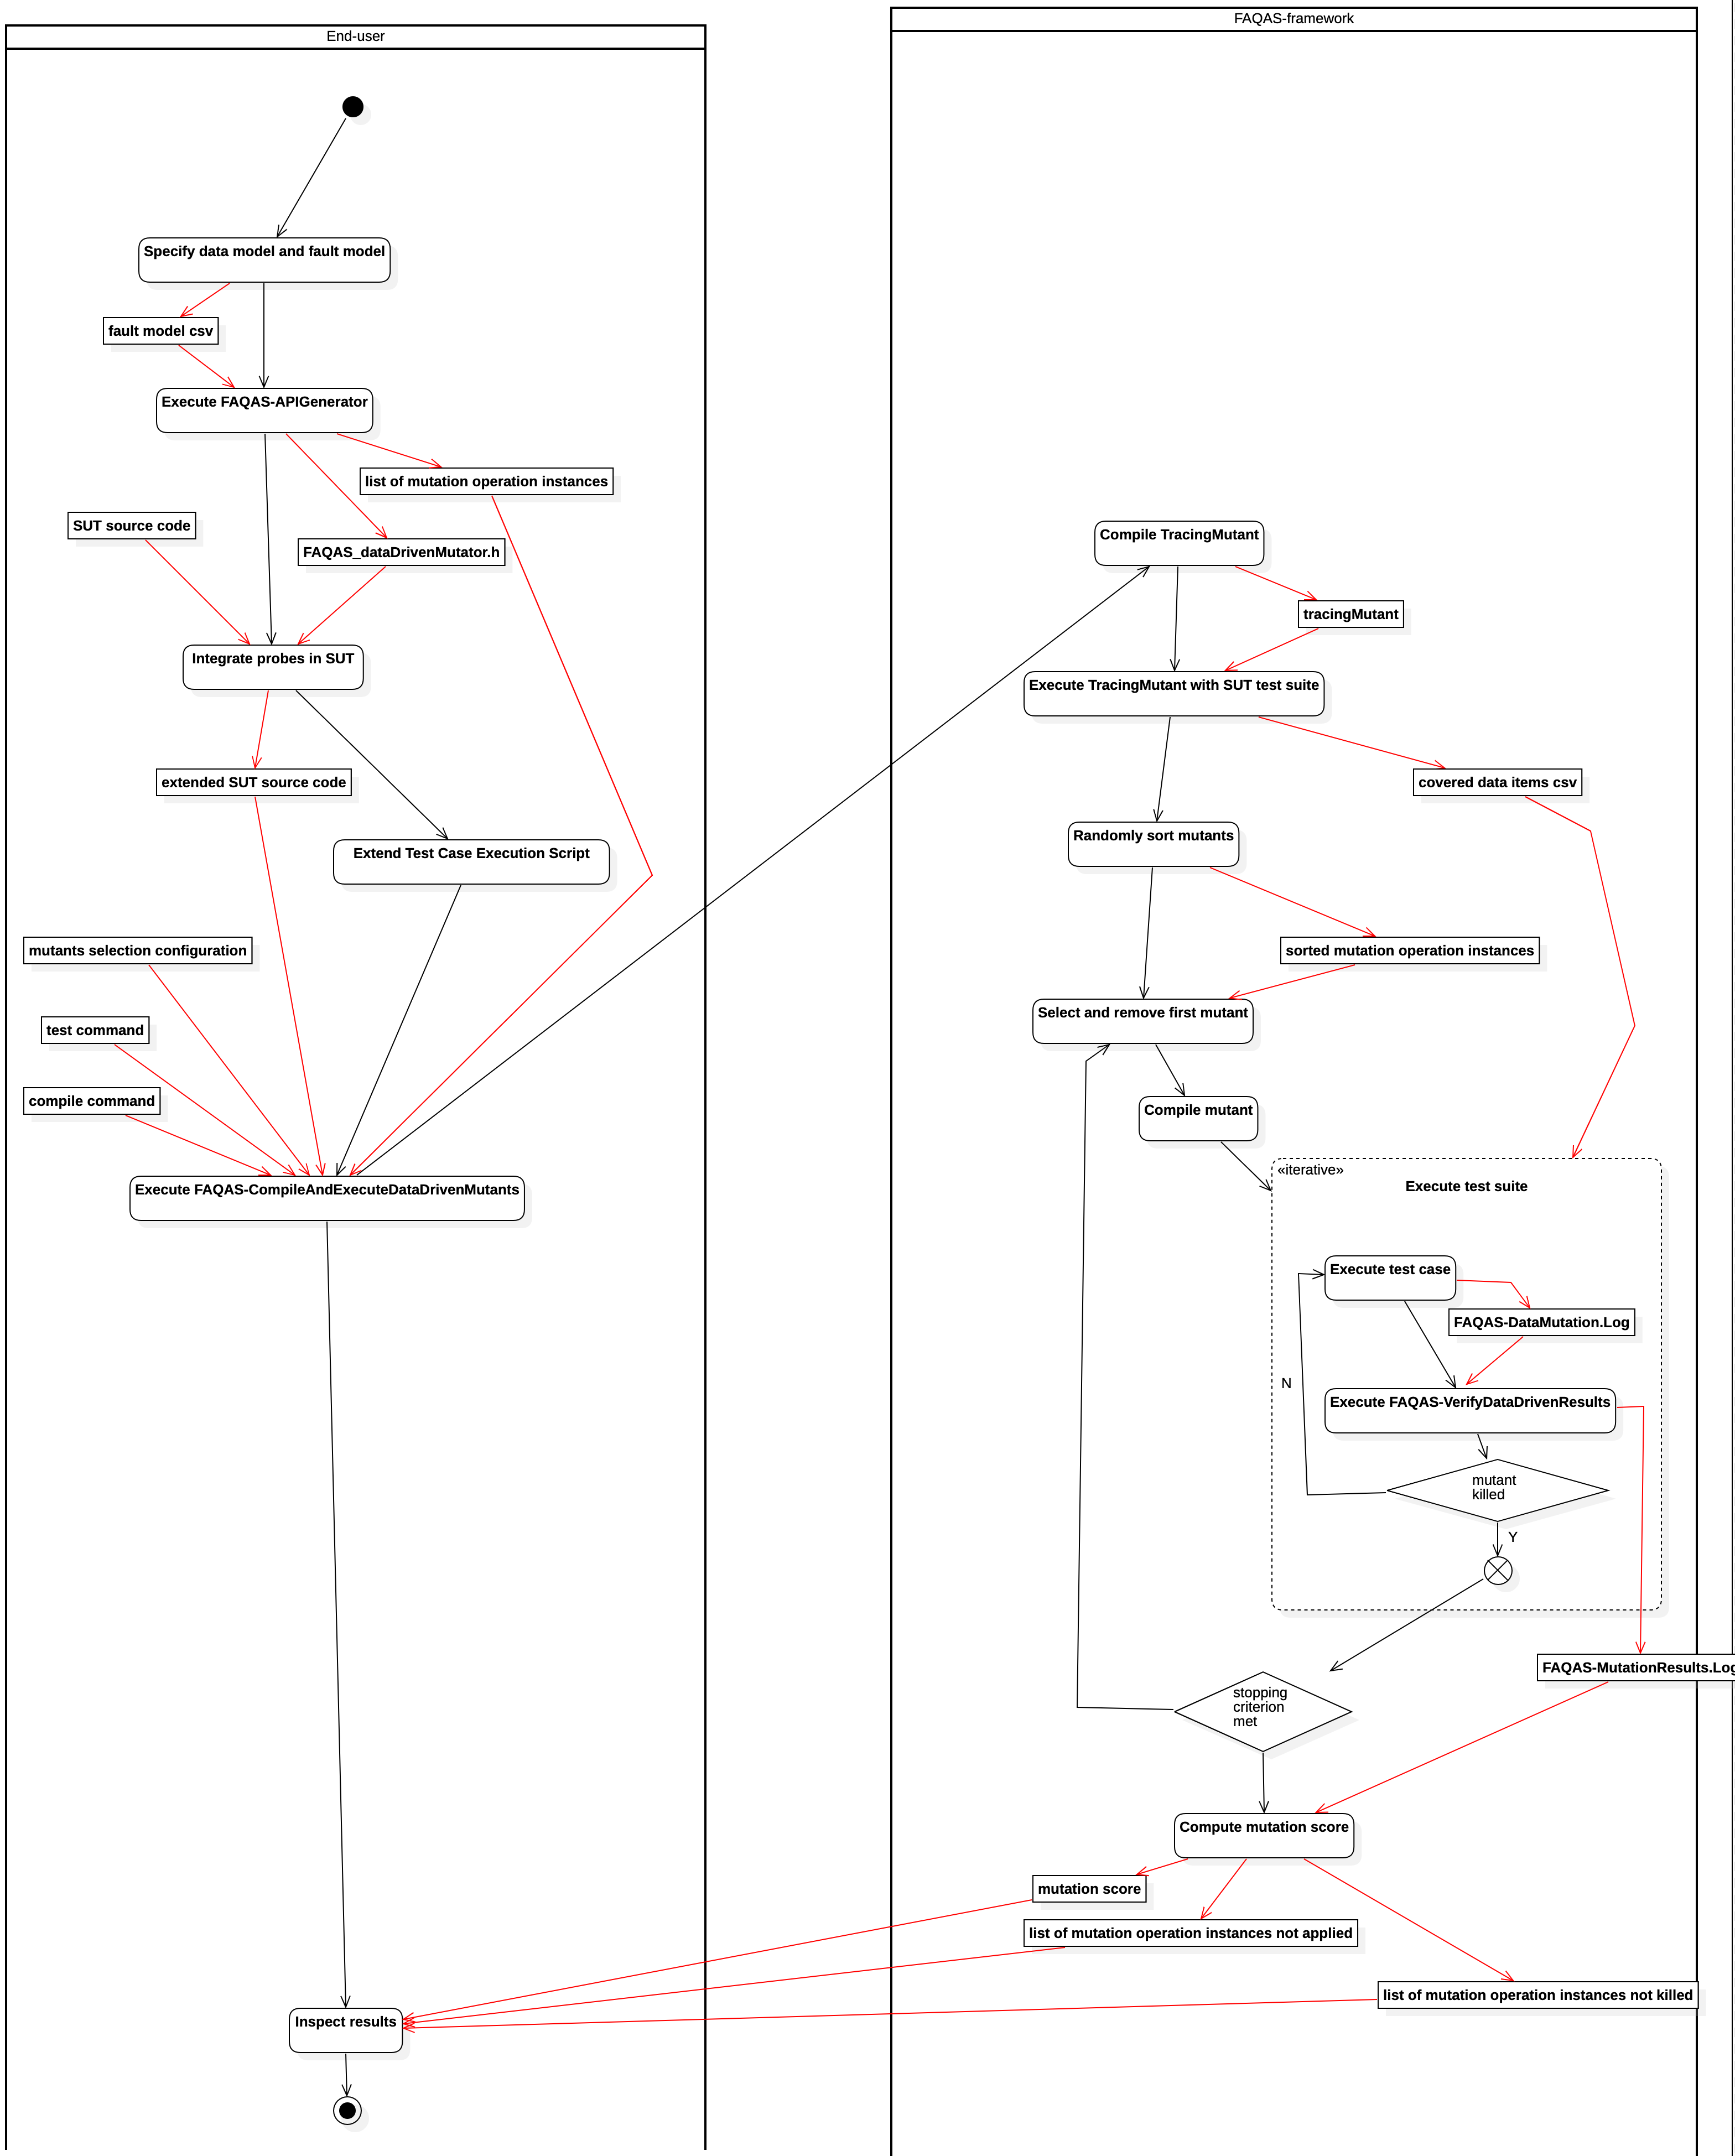
\includegraphics[width=\textwidth]{images/png/Activity1!DataDrivenTestSuiteEvaluation_3.png}
      \caption{Overview of the data-driven mutation testing process to evaluate test suite effectiveness.}
      \label{fig:process:dataDriven:evaluation}
\end{figure}

The data-driven mutation testing component shall implement the process for the evaluation of test suite effectiveness that is drafted in Figure~\ref{fig:process:dataDriven:evaluation}. Figure~\ref{fig:process:dataDriven:evaluation} relies on UML activity diagram notation. In Figure~\ref{fig:process:dataDriven:evaluation} the execution of specific software artefacts by the end-user is made explicit. Also, we use black arrows to draw control-flow, red arrows for data-flow. 

The activity \emph{Specify data model and fault model} in Figure~\ref{fig:process:dataDriven:evaluation} indicates that the engineer should prepare a csv file specifying the fault model and the data model for the SUT according to D2.

The activity \emph{Execute FAQAS-APIGenerator} in Figure~\ref{fig:process:dataDriven:evaluation} concerns the execution of the program \emph{Execute FAQAS-APIGenerator}.

The program \emph{FAQAS-APIGenerator} takes as input the \emph{fault model csv} and generates the file \emph{FAQAS\_dataDrivenMutator.h} and a csv file containing the \emph{list of mutation operation instances} derived from the fault model.

File \emph{FAQAS\_dataDrivenMutator.h} contains the FAQAS mutation testing API (i.e., the predefined functions to perform data mutation for buffers) and the fault model represented as a data structure. Details are provided in D2.

The activity \emph{Integrate probes in SUT} in Figure~\ref{fig:process:dataDriven:evaluation} indicates that the engineer should manually modify the source code of the SUT to integrate mutation probes into it. Examples are provided in \emph{Listing 2.3}, \emph{Listing 3.1}, and \emph{Appendix A - Section 1.1} of D2. 

The activity \emph{Extend Test Case Execution Script} in Figure~\ref{fig:process:dataDriven:evaluation} indicates that the engineer is expected to manually modify the scripts used to execute test cases so that they include an invocation to \emph{FAQAS-VerifyDataDrivenResults} after the execution of every single test case. 

The activity \emph{Execute FAQAS-CompileAndExecuteDataDrivenMutants} in Figure~\ref{fig:process:dataDriven:evaluation} concerns the execution of the program \emph{Execute FAQAS-CompileAndExecuteDataDrivenMutants}.

The program \emph{Execute FAQAS-CompileAndExecuteDataDrivenMutants} receives as inputs the command to compile the SUT, the command to execute the test suite, the path to the extended SUT source code, and the mutants selection configuration. It automatically executes a number of activities required to compute the mutation score: \emph{Compile TracingMutant}, \emph{Execute TracingMutant with SUT test suite}, \emph{Randomly sort mutants}, \emph{Select and remove first mutant}, \emph{Compile mutant}, \emph{Execute test suite},  \emph{Compute mutation score}.

The program \emph{FAQAS-CompileAndExecuteDataDrivenMutants} implements the four mutants selection strategies: \emph{all mutants} (i.e., all the mutants are tested), \emph{proportional uniform sampling} (i.e., a subset of the mutants is tested selected based on a percentage), \emph{uniform fixed-size sampling} (i.e., a subset of the mutants is tested selected based on a fixed number), and \emph{uniform FSCI sampling} (i.e., a subset of the mutants is tested, they are selected according to the FSCI criterion).

The \emph{mutants selection configuration} indicates the mutants selection strategy and a configuration value that specifies the number of mutants to consider; the value may indicate the percentage of mutants to sample (for \emph{proportional uniform sampling}), the number of mutants to sample (for \emph{uniform fixed-size sampling}), or the size of the confidence interval (for \emph{uniform FSCI sampling}).

The activity \emph{Compile TracingMutant} indicates that the system compiles a version of the SUT that traces the data items (targeted by mutation) that are covered by each test case (see D2, Figure 2.9, line 5).

The activity \emph{Execute TracingMutant with SUT test suite} indicates that the system executes the SUT test suite. Since the test suite is executed with the TracingMutant it leads to the generation of a csv files that indicates, for every test case, the data items being exercised by the test case.

The activity \emph{Randomly sort mutants} indicates that  \emph{FAQAS-CompileAndExecuteDataDrivenMutants} generates a randomly sorted list of mutation operation instances. This list is derived from the \emph{list of mutation operation instances}.

The activity \emph{Select and remove first mutant} indicates that  \emph{FAQAS-CompileAndExecuteMutants} selects the first item in the \emph{sorted mutation operation instances} and removes it from the list.

The activity \emph{Compile mutant} indicates that the system compiles a version of the SUT with the selected mutation operation instance enabled.

The activity \emph{Execute test case} indicates that the test suite of the SUT executes a test case. Only the test cases exercising the data item targeted by the mutation operator are executed. Since the test case is executed against the mutated SUT, if the mutation operation is performed, then the file \emph{FAQAS-MutationResults.Log} will be created (this is a feature of the FAQAS data-driven mutation API).

File \emph{FAQAS-MutationResults.Log} contains the ID of the mutation operation instance applied.

Program \emph{FAQAS-VerifyDataDrivenResults} receives as input the ID of the test case and  the status of a test case (i.e., PASS or FAIL). It checks if a data mutation operator has been applied based on the content of \emph{FAQAS-DataMutation.Log}. It deletes \emph{FAQAS-DataMutation.Log}. It updates the content of \emph{FAQAS-MutationResults.Log}.

If program \emph{FAQAS-VerifyDataDrivenResults} determines that a mutation operation instance has been killed, then the test suite execution is terminated.

File \emph{FAQAS-MutationResults.Log} indicates, for every executed test case, the ID of the mutation operation instance applied and the mutation result (KILLED or LIVE). A test case may appear multiple times in this file, each time with a different mutation operation instance ID associated.

The execution of the test suite is repeated till a termination criterion is met. The termination criterion depends on the mutants selection strategy:
\begin{itemize}
\item \emph{all mutants}: the list \emph{sorted list of mutants} is empty
\item \emph{proportional uniform sampling}: a number of mutants matching the selected percentage has been executed
\item \emph{uniform fixed-size sampling}: a number of mutants matching the selected value has been executed
\item \emph{uniform FSCI sampling}: the confidence interval computed from \emph{mutation results csv} is smaller than the length specified by the user.
\end{itemize}

The activity \emph{Compile mutation score} concerns the computation of the mutation score based on the mutation results reported in \emph{FAQAS-MutationResults.Log}. The formula is provided in D2. As output of the computation of the mutation score the system reports also the \emph{list of mutation operation instances not killed} and the \emph{list of mutation operation instances not applied}. The \emph{list of mutation operation instances not killed} includes also the name of test cases executed for each, to facilitate the improvement of the test suite.

The end-user inspects the \emph{list of mutation operation instances not applied} to understand which data types had not been covered by the test suite. The end-user inspects the \emph{list of mutation operation instances not killed} to understand which test cases need improvement.


\subsection{Data-Driven Test Suite Augmentation}

\begin{figure}[]
  \centering
	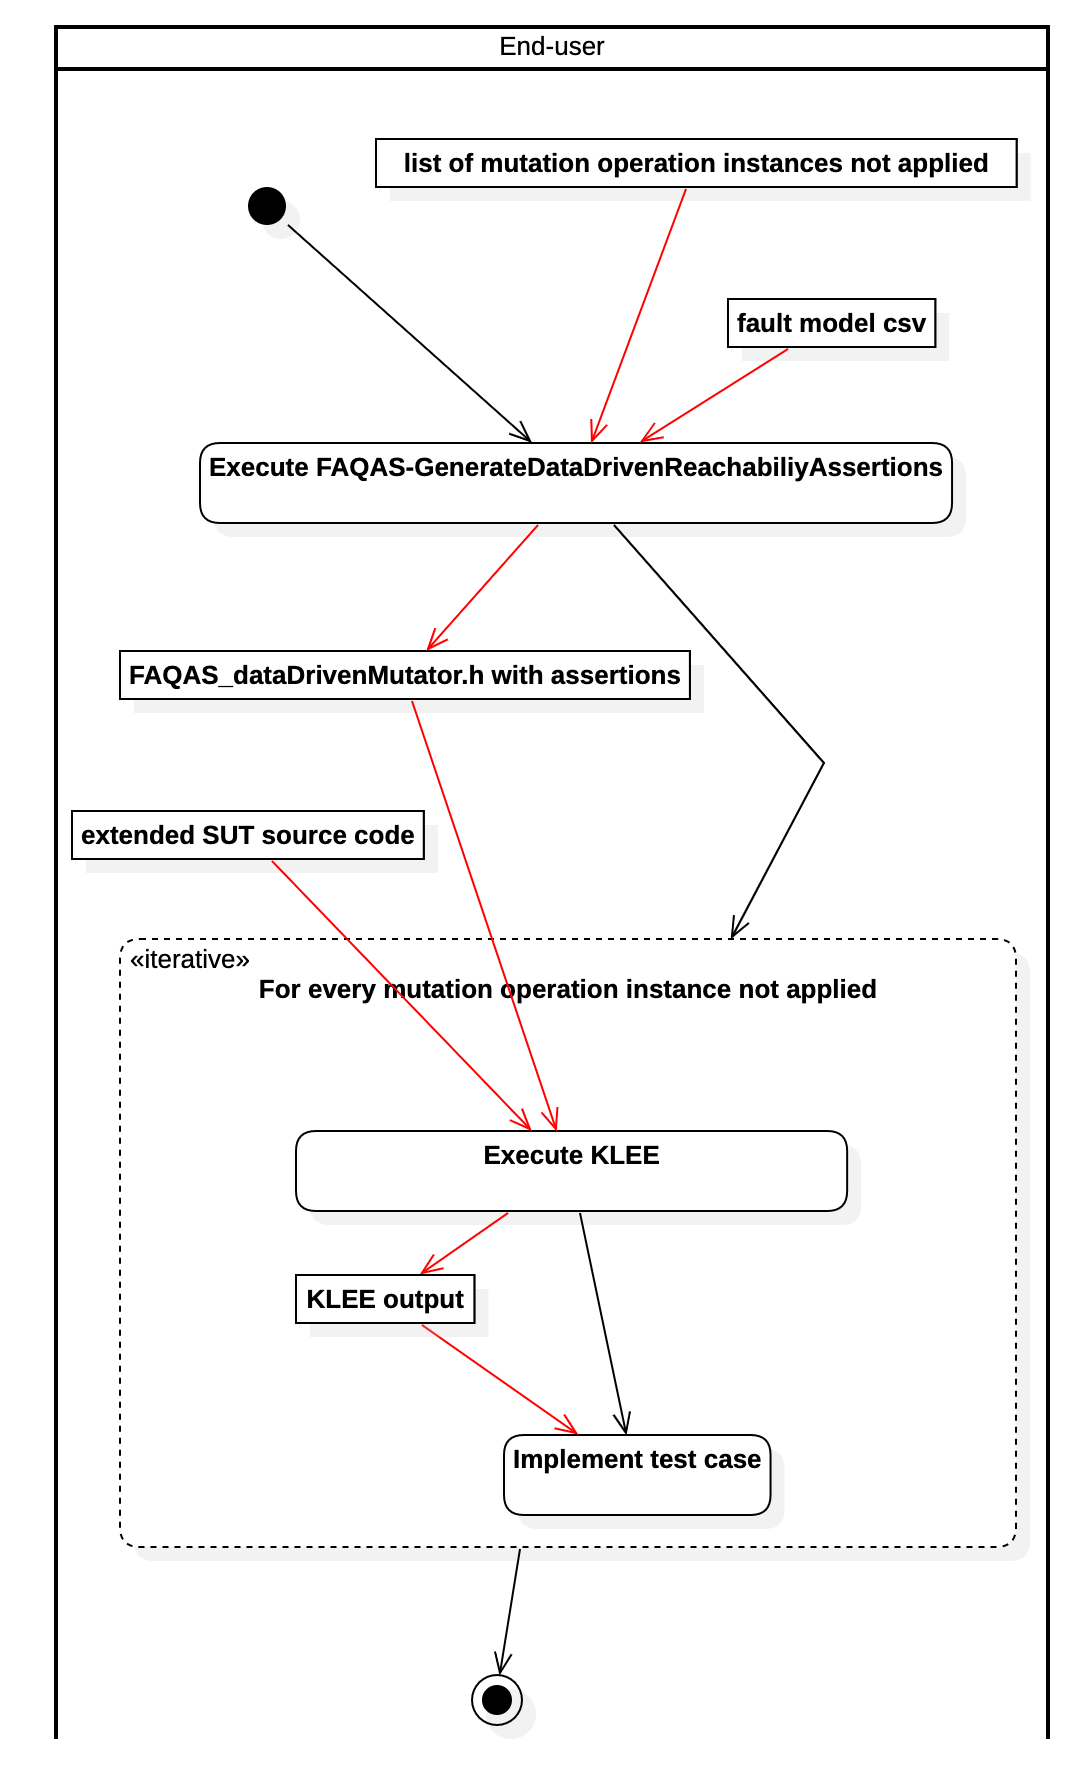
\includegraphics[width=0.4\textwidth]{images/png/Activity1!DataDrivenTestSuiteAugmentation_4.png}
      \caption{Overview of the data-driven test suite augmentation process.}
      \label{fig:process:dataDriven:augment}
\end{figure}

The activity \emph{Execute FAQAS-GenerateDataDrivenReachabiliyAssertions} in Figure~\ref{fig:process:dataDriven:augment} concerns the execution of the program \emph{Execute FAQAS-GenerateDataDrivenReachabiliyAssertions}.

The program \emph{FAQAS-GenerateDataDrivenReachabiliyAssertions} takes as input the fault model and generates a version of \emph{FAQAS\_dataDrivenMutator.h} that contains reachability assertions that enable KLEE to generate inputs that reach the mutation.

The activity \emph{Execute KLEE} indicates that the end-user should execute KLEE, after performing the required scaffolding, if necessary. A methodological procedure document to support the end-user will be provided.

The activity \emph{Implement test case} indicates that the end-user should implement a test case based on KLEE's output.

